\documentclass{article}
\usepackage[utf8]{inputenc} % Allow more characters
\usepackage{graphicx} % images
\usepackage{xcolor}
\usepackage{listings} % code quotes
\lstset{
  basicstyle=\ttfamily,
  columns=fullflexible,
  frame=single,
  breaklines=true,
  postbreak=\mbox{\textcolor{red}{$\hookrightarrow$}\space},
}

\title{Relatório de Trabalho Prático}
\author{David Pires nº37272 e Pedro Maria nº39866}
\date{Janeiro 2020}

\begin{document}

\begin{titlepage}
    \maketitle

    
\includegraphics[scale=0.5]{logo_ubi_vprincipal.jpg}

\end{titlepage}

\section{Conteúdo}

\tableofcontents

\newpage

\section{Motivação}

A grande motivação deste projeto foi conseguir de certa forma criar um robô que seja mais inteligente que o robô comum, pois estes não são capazes de reconhecer os objetos presentes no meio, retirar informações e fazer conclusões acerca do mesmo. Sendo então o objetivo deste trabalho desenvolver então essas capacidades.

\section{Objetivos}

O objetivo deste trabalho é a criação de um programa que consiga comandar um robô móvel num determinado ambiente e que este seja capaz não só de reconhecer o ambiente que o rodeia mas também responder a perguntas específicas sobre o mundo em que está inserido tendo em conta a informação que o robô recolheu até ao dado momento.

\newpage

\section{Implementação}

\subsection{Variáveis auxiliares}

\paragraph{Para a conclusão deste trabalho, recorremos à criação de várias variáveis auxiliares, para o manuseamento das informações obtidas pelo robô e pedidas pelo utilizador do programa.}

\subsubsection{Lista das salas}
\begin{lstlisting}[language=Python]
room_list = [(1,-15.6,-3.0,-3.6,-0.8), (2,-12.0,-1.4,-8.9,4.8), (3,-10.6,4.8,3.6,7.9), (4,-4.6,-0.8,-0.8,4.8), (5,-15.6,-1.4,-12.5,3.0), (6,-15.6,3.0,-12.5,7.9), (7,-15.6,7.9,-10.6,11.1), (8,-10.6,7.9,-5.6,11.1), (9,-5.6,7.9,-0.5,11.1), (10,-0.5,7.9,3.6,11.1), (11,-0.8,1.4,3.6,4.8), (12,-0.8,-0.8,3.6,1.4), (13,-8.9,-0.8,-6.5,4.8),(14,-6.5,-0.8,-4.6,4.8)]
\end{lstlisting}

Esta é uma lista pré definida no programa que contem as coordenadas de cada sala. Esta lista é composta por tuplos do tipo (roomNumber, x1, y1, x2, y2) em que roomNumber corresponde ao numero da sala, x1 e y1, correspondem às coordenadas do canto inferior esquerdo da sala e x2, y2, corresponde às coordenadas do canto superior direito da sala.

\subsubsection{Lista de objetos}
\begin{lstlisting}[language=Python]
object_list = []
\end{lstlisting}  

Esta é uma lista, que é incrementada dinamicamente à medida que o robô descobre um novo objeto. Esta lista será composta por tuplos, com a seguinte estrutura: (roomNumber, objectName, objectID), em que roomNumber corresponde ao numero da sala onde foi encontrado o objeto, objectName corresponde ao nome do objecto e objectID corresponde ao seu ID.

\subsubsection{Lista de pontos de interesse}
\begin{lstlisting}[language=Python]
point_list = []
\end{lstlisting}

Esta é uma lista incrementada dinamicamente com pontos de interesse, que neste caso se podem traduzir em "portas" (menos nos casos se passagem de um corredor para outro).
Esta lista é composta por tuplos, com a seguinte estrutura: (uuid, x, y, roomA, roomB), onde:
\newline - uuid é um ID único aleatoriamente gerado, representante deste ponto. 
\newline - x e y são as coordenadas do ponto.
\newline - roomA e roomB são as salas entre o ponto (visto que este é um ponto correspondente à passagem de uma sala para outra).

\subsubsection{Garfo dos pontos de interesse}
\begin{lstlisting}[language=Python]
  from collections import defaultdict

  class Graph():
      def __init__(self):
          self.edges = defaultdict(list)
          self.weights = {}
      
      def add_edge(self, from_node, to_node, weight):
          self.edges[from_node].append(to_node)
          self.edges[to_node].append(from_node)
          self.weights[(from_node, to_node)] = weight
          self.weights[(to_node, from_node)] = weight
  
      def getWeight(self, from_node, to_node):
          return self.weights[(from_node, to_node)]  
\end{lstlisting}
\begin{lstlisting}[language=Python]
graph = Graph()
\end{lstlisting}

Para isto trabalhamos numa classe feita originalmente por Ben Keen (Link na Bibliografia). Este é um grafo bi-dirigido com pesos, em que cada peso corresponde à distância de um ponto ao outro e as ligações corresponderão a pontos possíveis de alcançar sem paredes como obstáculos. Cada nodo é um uuid, representante de um ponto na lista de pontos.

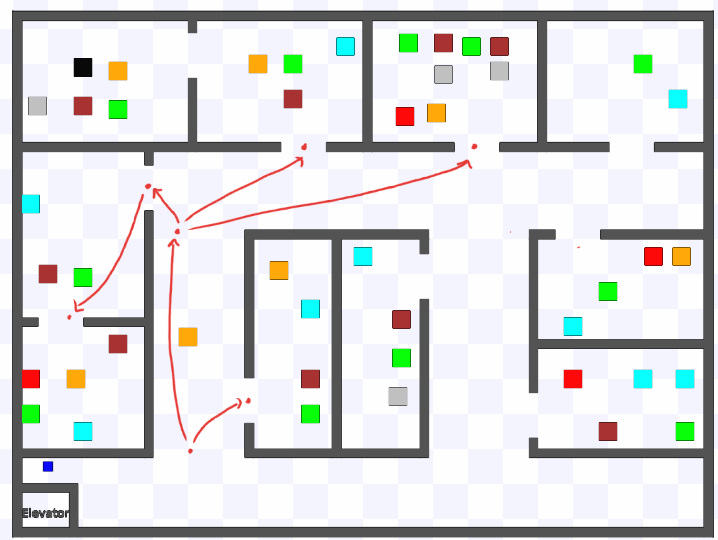
\includegraphics[scale=0.4]{rosexample.png}

\newpage
\subsection{Funções auxiliares}  
  
\paragraph{Neste trabalho recorremos à criação de várias funções auxiliares, de forma a facilitar o nosso trabalho. Aqui vamos explicar algumas dessas funções.}

\subsubsection{Calcular a distância entre dois pontos (x1, y1) e (x2, y2)}
\begin{lstlisting}[language=Python]
    import math

    def calculateDistance(x1, y1, x2, y2):
        dx = x2-x1
        dy = y2-y1
        distance = math.sqrt((dx**2) + (dy**2))
        return distance
\end{lstlisting}

Esta função localiza-se no ficheiro CoordHelper.py (Decidimos criar este ficheiro separado, para caso, venha a ser necessário criar mais funções auxiliares relacionadas com Coordenas) e retorna um valor que representa a distância entre dois pontos no plano x, y.

\subsubsection{Registo de um novo ponto de interesse}
\begin{lstlisting}[language=Python]
  def new_point(coordX, coordY, roomA, roomB):
	uid = uuid.uuid4()
	point_list.append((uid, coordX, coordY, roomA, roomB))
	for point in point_list:
		if point[3] == roomA or point[3] == roomB or point[4] == roomA or point[4] == roomB:
			distance = CoordHelper.calculateDistance(point[1], point[2], coordX, coordY)
			graph.add_edge(uid, point[0], distance)
\end{lstlisting}

Esta função é chamada sempre que o robô passa de uma sala para outra. Esta usa a biblioteca uuid para gerar um novo uuid, e guarda os dados na lista de pontos e para cada ponto de interesse alcançável sem obstáculos, calcula a distância e adiciona uma ponte no grafo.

\subsubsection{Algoritmo dijsktra}
\begin{lstlisting}[language=Python]
  def dijsktra(graph, initial, end):
  # shortest paths is a dict of nodes
  # whose value is a tuple of (previous node, weight)
  shortest_paths = {initial: (None, 0)}
  current_node = initial
  visited = set()
  
  while current_node != end:
      visited.add(current_node)
      destinations = graph.edges[current_node]
      weight_to_current_node = shortest_paths[current_node][1]

      for next_node in destinations:
          weight = graph.weights[(current_node, next_node)] + weight_to_current_node
          if next_node not in shortest_paths:
              shortest_paths[next_node] = (current_node, weight)
          else:
              current_shortest_weight = shortest_paths[next_node][1]
              if current_shortest_weight > weight:
                  shortest_paths[next_node] = (current_node, weight)
      
      next_destinations = {node: shortest_paths[node] for node in shortest_paths if node not in visited}
      if not next_destinations:
          return "Route Not Possible"
      # next node is the destination with the lowest weight
      current_node = min(next_destinations, key=lambda k: next_destinations[k][1])
  
  # Work back through destinations in shortest path
  path = []
  while current_node is not None:
      path.append(current_node)
      next_node = shortest_paths[current_node][0]
      current_node = next_node
  # Reverse path
  path = path[::-1]
  return path
\end{lstlisting}

Para isto usamos o código feito por Ben Keen (Link na Bibliografia). Esta função retornará uma lista de pontos, que representará o menor caminho a percorrer para ir de um ponto até outro.

\newpage
\subsection{Resposta às perguntas}

\subsubsection{Pergunta 1: How many rooms are not occupied?}
\begin{lstlisting}[language=Python]
  def question1():
	counterOccuped = 0
	counterNotKnown = 0
	for roomNumber in range(5, len(room_list) + 1):
		counterObj = 0
		for obj in object_list:
			if obj[0] == roomNumber:
				counterObj += 1
				if obj[1] == "person":
					counterOccuped += 1
		if counterObj == 0:
			counterNotKnown += 1
	print( " There are %d rooms not occuped by people in %d known rooms. " % (((10 - counterNotKnown) - counterOccuped), (10 - counterNotKnown)) ) 
\end{lstlisting}

Para responder a esta pergunta é feita uma análise a todas as salas que o robô conhece e para cada uma das salas vai ser verificado se há pelo menos uma pessoa em cada sala ou não, havendo assim uma contagem das salas que estão ocupadas por pessoas.

\subsubsection{Pergunta 2: How many suites did you find until now?}
\begin{lstlisting}[language=Python]
  def question2():
	counter = 0
	for roomNumber in range(1, len(room_list) + 1):
		if (getRoomType(roomNumber) == "Suite room"):
			counter += 1
	print( " I've found %d Suite rooms so far. " % counter )
\end{lstlisting}

Para responder a esta pergunta é feita uma análise a todas a salas que o robô conhece e todas aquelas que forem do tipo "Suite room", e então retornamos a contagem das mesmas.

\subsubsection{Pergunta 3: Is it more probable to find people in the corridors or inside the rooms?}
\begin{lstlisting}[language=Python]
  def question3():
	counterHall = 0
	counterRooms = 0
	for obj in object_list:
		if obj[1] == "person":
			if obj[0] <= 4:
				counterHall += 1
			else:
				counterRooms += 1
	if counterHall > counterRooms:
		print( " Is more likely to meet people in the halls. " )
	elif counterHall < counterRooms:
		print( " Is more likely to meet people in the rooms. " )
	elif counterHall == 0 and counterRooms == 0:
		print ( "I don't know any person yet. " )
	else:
		print( " The probability of find people in rooms or in the halls is equal. " )
\end{lstlisting}

Para responder a esta pergunta contamos o número de pessoas nos corredores e o número de pessoas nas salas, comparamos os dois valores e retornamos resultado dessa comparação.

\subsubsection{Pergunta 4: If you want to find a computer, to which type of room do you go to?}
\begin{lstlisting}[language=Python]
  def question4():
	roomNumber = -1
	for obj in object_list:
		if obj[1] == "computer":
			if getRoomType(obj[0]) == "Meeting room" or getRoomType(obj[0]) == "Generic room": # Only for privacy :)  
				roomNumber = obj[0]
				break
			roomNumber = obj[0]
	if roomNumber == -1:
		print( " I don't know any room with a computer. " )
	else:
		print( " Go to room number %d to find a Computer. " % roomNumber )
\end{lstlisting}

Para responder a esta pergunta apenas se vai verificar em todas as salas que o robô conhece quais contêm computadores e retornamos uma sala que contenha então um computador.

\subsubsection{Pergunta 5: What is the number of the closest single room?}
\begin{lstlisting}[language=Python]
  def closestSingleRoom(atualX, atualY):
	min_room = -1
	min_distance = 9999999
	for room in room_list:
		if (getRoomType(room[0]) == "Single room"):
			tempDistance = calculateDistance(atualX, atualY, dijsktraRooms(match_room(atualX, atualY), room[0]))
			if (tempDistance < min_distance):
				min_distance = tempDistance
				min_room = room[0]
	return min_room

def question5():
	csr = closestSingleRoom(x_ant, y_ant)
	if csr != -1:
		print("The closest Single room is %d." % csr)
	else:
		print("I don't know any Single room yet.")
\end{lstlisting}

Para responder a esta pergunta recorremos ao cálculo da distância de onde o robô está até cada Single room conhecida, calculando o menor caminho para cada Single room com o algoritmo dijsktra e comparando as distâncias.
Assim retornará a Single room mais perto (com menor distância, a andar).

\subsubsection{Pergunta 6: How can you go from the current room to the elevator?}
\begin{lstlisting}[language=Python]
  def question6():
	roomPath = getRoomPath(dijsktraRooms(match_room(x_ant, y_ant), -1), match_room(x_ant, y_ant))
	roomPath = roomPath[1:-1]
	result = " Visit the follow rooms to go to the Elevator: "
	for room in roomPath:
		result += str(room) + "  "
	print(result)
\end{lstlisting}

Para responder a esta pergunta usamos o algoritmo dijsktra para caulcular o menor caminho desde a sala atual do robô até ao elevador (representado como a sala -1). Retornamos uma lista ordenada das salas a visitar até chegar ao elevador.

\subsubsection{Pergunta 7: How many books do you estimate to find in the next 2 minutes?}
\begin{lstlisting}[language=Python]
  startTime = time.time()
\end{lstlisting}
\begin{lstlisting}[language=Python]
  def question7():
	actualTime = time.time()
	counterBooks = 0
	for obj in object_list:
		if obj[1] == "book":
			counterBooks += 1
	result = (120 * counterBooks) / (actualTime - startTime)
	print( " I think I will find %d books in the next 2 minutes. " % int(result))
\end{lstlisting}

Para responder a esta pergunta recorremos à biblioteca time, guardando no inicio do programa o tempo o tempo de inicio, e cada vez que for feita esta questão um tempo. Para responder à pergunta será dada uma resposta com base no seguinte cálculo:
\newline (120 * numberOfBooks) / timeInterval
\newline Em que, numberOfBooks corresponde ao numero de livros encontrados pelo robô até agora e timeInterval corresponde ao tempo decorrido em segundos desde o inicio do programa.

\subsubsection{Pergunta 8: What is the probability of finding a table in a room without books but that
has at least one chair?}
\begin{lstlisting}[language=Python]
  def question8():
	counterRoomWithChairAndNotBook = 0
	counterRoomWithTableAndChairAndNotBook = 0
	for room in range(5, 14):
		counterBook = 0
		counterChair = 0
		counterTable = 0
		for obj in object_list:
			if obj[0] == room:
				if obj[1] == "chair":
					counterChair += 1
				if obj[1] == "book":
					counterBook += 1
				if obj[1] == "table":
					counterTable += 1
		if counterChair > 0 and counterBook == 0:
			counterRoomWithChairAndNotBook += 1
		if counterChair > 0 and counterTable > 0 and counterBook == 0:
			counterRoomWithTableAndChairAndNotBook += 1
	if counterRoomWithChairAndNotBook == 0:
		print( " I don't know any room without books but that has at least one chair yet. " )
	else:
		result = counterRoomWithTableAndChairAndNotBook / counterRoomWithChairAndNotBook
		print( " The probability of finding a table in a room without books but that has at least one chair is %d. " % result )
\end{lstlisting}

Para responder a esta pergunta usamos a Regra de Bayes, calculando \[P(T | C, ~B)\] em que:
\newline - T corresponde à probabibilidade de encontrar uma o mais Mesas em uma sala.
\newline - C corresponde à probabibilidade de encontrar uma o mais Cadeiras em uma sala.
\newline - B corresponde à probabibilidade de encontrar um o mais Livros em uma sala.
\newline \[P(T | C, ~B)\] Coresponde à probabibilidade de encontrar uma ou mais mesas em uma sala sabendo que contem uma ou mais cadeiras e não contem livros. 

\newpage
\section{Conclusão}

\paragraph{Com este trabalho concluímos que mesmo para um ambiente controlado podem surgir algumas dificuldades em questões que aparentam ser simples, e que assim sendo serão ainda mais complicadas de implementar no mundo real. }

\subsection{Partição do trabalho}

Perguntas 1 a 4: Pedro Maria
\newline Perguntas 5 a 8: David Pires
\newline Relatório:
\newline Motivação, Objetivos e Conclusão: Pedro Maria
\newline Perguntas 1 a 4: Pedro Maria
\newline Perguntas 5 a 8: David Pires
\newline Apresentação: Pedro Maria

\section{Bibliografia}

- http://benalexkeen.com/implementing-djikstras-shortest-path-algorithm-with-python/

\end{document}